\chapter{团队成员分工描述}

\underline{刘格伦}
\begin{itemize}
    \item 实现红外温度到可视颜色的伪彩色编码转换
    \item 建立服务器,对收到的数据进行处理
    \item 实现热成像图的绘制
    \item 实现前后端的通信
    \item 前端页面的美化
    \end{itemize}
\begin{figure}[htbp]
        \centering
        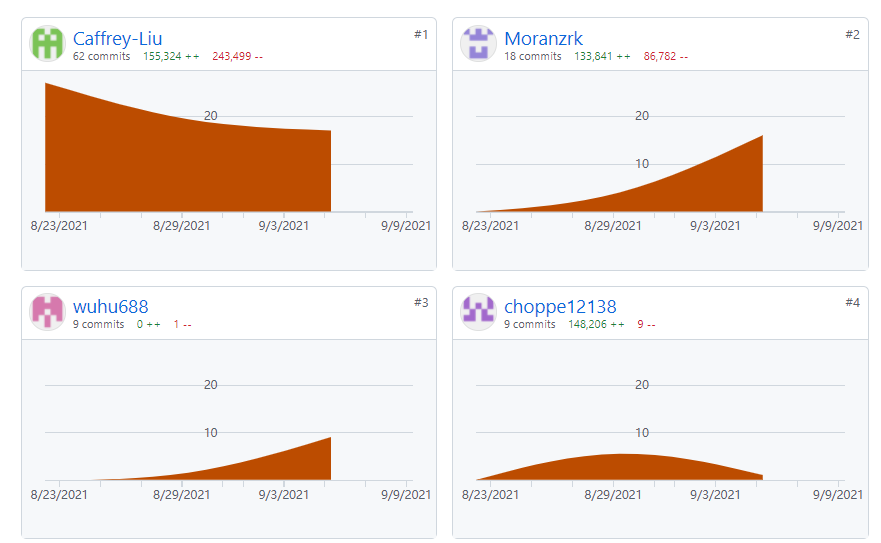
\includegraphics[width=0.5\textwidth]{github.png}
        \caption{刘格伦githubcommit截图}\label{fig:github}
        \vspace{\baselineskip}
        \end{figure}
\underline{郑睿恺}
\begin{itemize}
    \item 实现ESP32和红外传感器的数据采集方案
    \item 实现和改进ESP32的Wi-Fi通信
    \item 实现二元和三元插值算法
    \item LaTex文档的编写
    \item 数据库函数的封装
    \end{itemize}
    \begin{figure}[htbp]
        \centering
        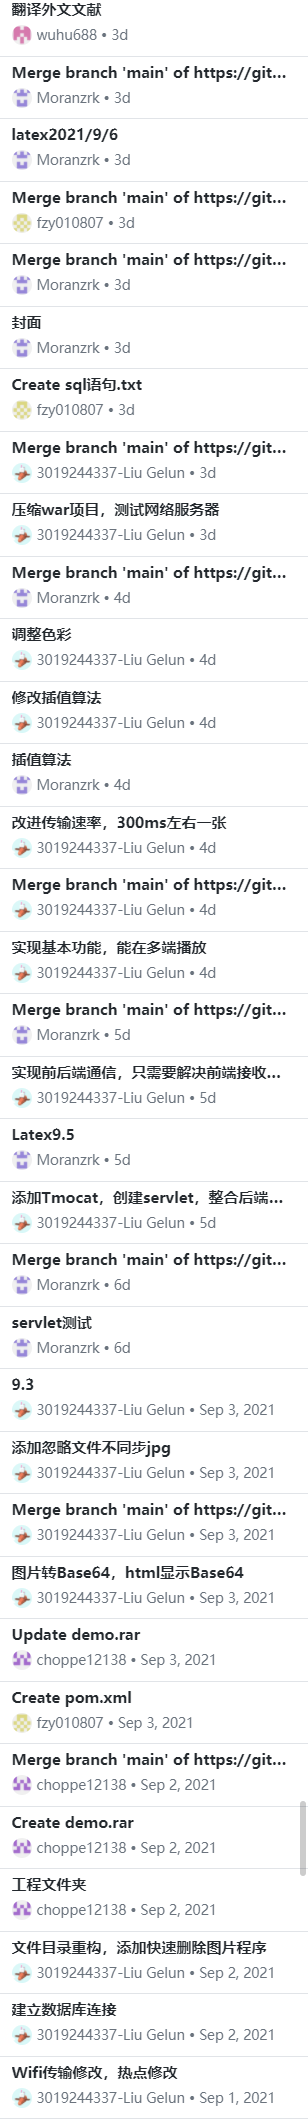
\includegraphics[width=0.5\textwidth]{github2.png}
        \caption{郑睿恺githubcommit截图}\label{fig:github2}
        \vspace{\baselineskip}
        \end{figure}



        
\underline{樊振宇}
\begin{itemize}
    \item 数据库的建立,sql语句的编写
    \item 协助完成LaTeX文档的编写
    \end{itemize}
    \begin{figure}[htbp]
        \centering
        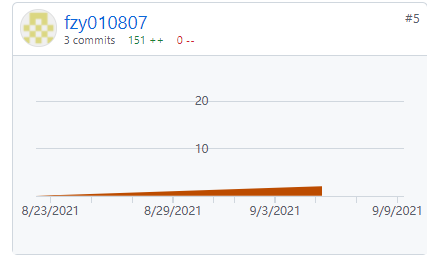
\includegraphics[width=0.5\textwidth]{github5.png}
        \caption{樊振宇githubcommit截图}\label{fig:github}
        \vspace{\baselineskip}
        \end{figure}
    \underline{周子涵}
\begin{itemize}
    \item 协助完成前端页面
    \item 协助完成LaTeX文档的编写
    \end{itemize}
    \begin{figure}[htbp]
        \centering
        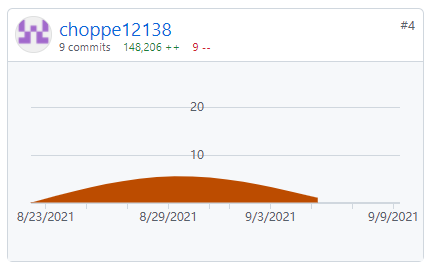
\includegraphics[width=0.5\textwidth]{github4.png}
        \caption{周子涵githubcommit截图}\label{fig:github4}
        \vspace{\baselineskip}
        \end{figure}
    \underline{李世军}
\begin{itemize}
    \item 英文文献的翻译
    \item 协助完成LaTeX文档的编写
    \end{itemize}
    \begin{figure}[htbp]
        \centering
        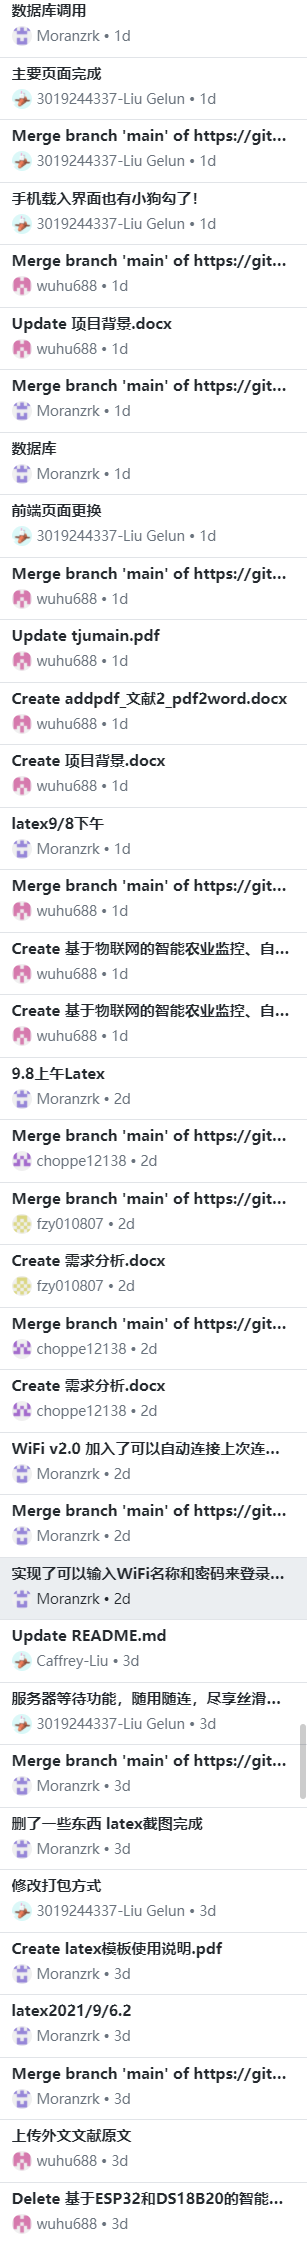
\includegraphics[width=0.5\textwidth]{github3.png}
        \caption{李世军githubcommit截图}\label{fig:github3}
        \vspace{\baselineskip}
        \end{figure}
    
      







